\section{Viden}

\subsection{State Of The Art}
\begin{frame}{State Of The Art}
	Find concept from existing systems
	Hvilke fandt vi og hvilke concepter differencerede dem.
\end{frame}
\subsection{Interviews og Informanter}
\begin{frame}{Interviews og Informanter}
	Hvem de var som interresanter, hvor vi fandt dem og hvordan vi afviklede interviewsne

	1 iteration: state of the art
	2 iteration: interview med forskellige barer og gæster
	3 iteration: vertical prototype med fabrikken
	4 iteration: usability test på en telefon, explicit
\end{frame}
\subsection{Prototyper}
\begin{frame}{Prototyper}
	\begin{figure}
		\centering
		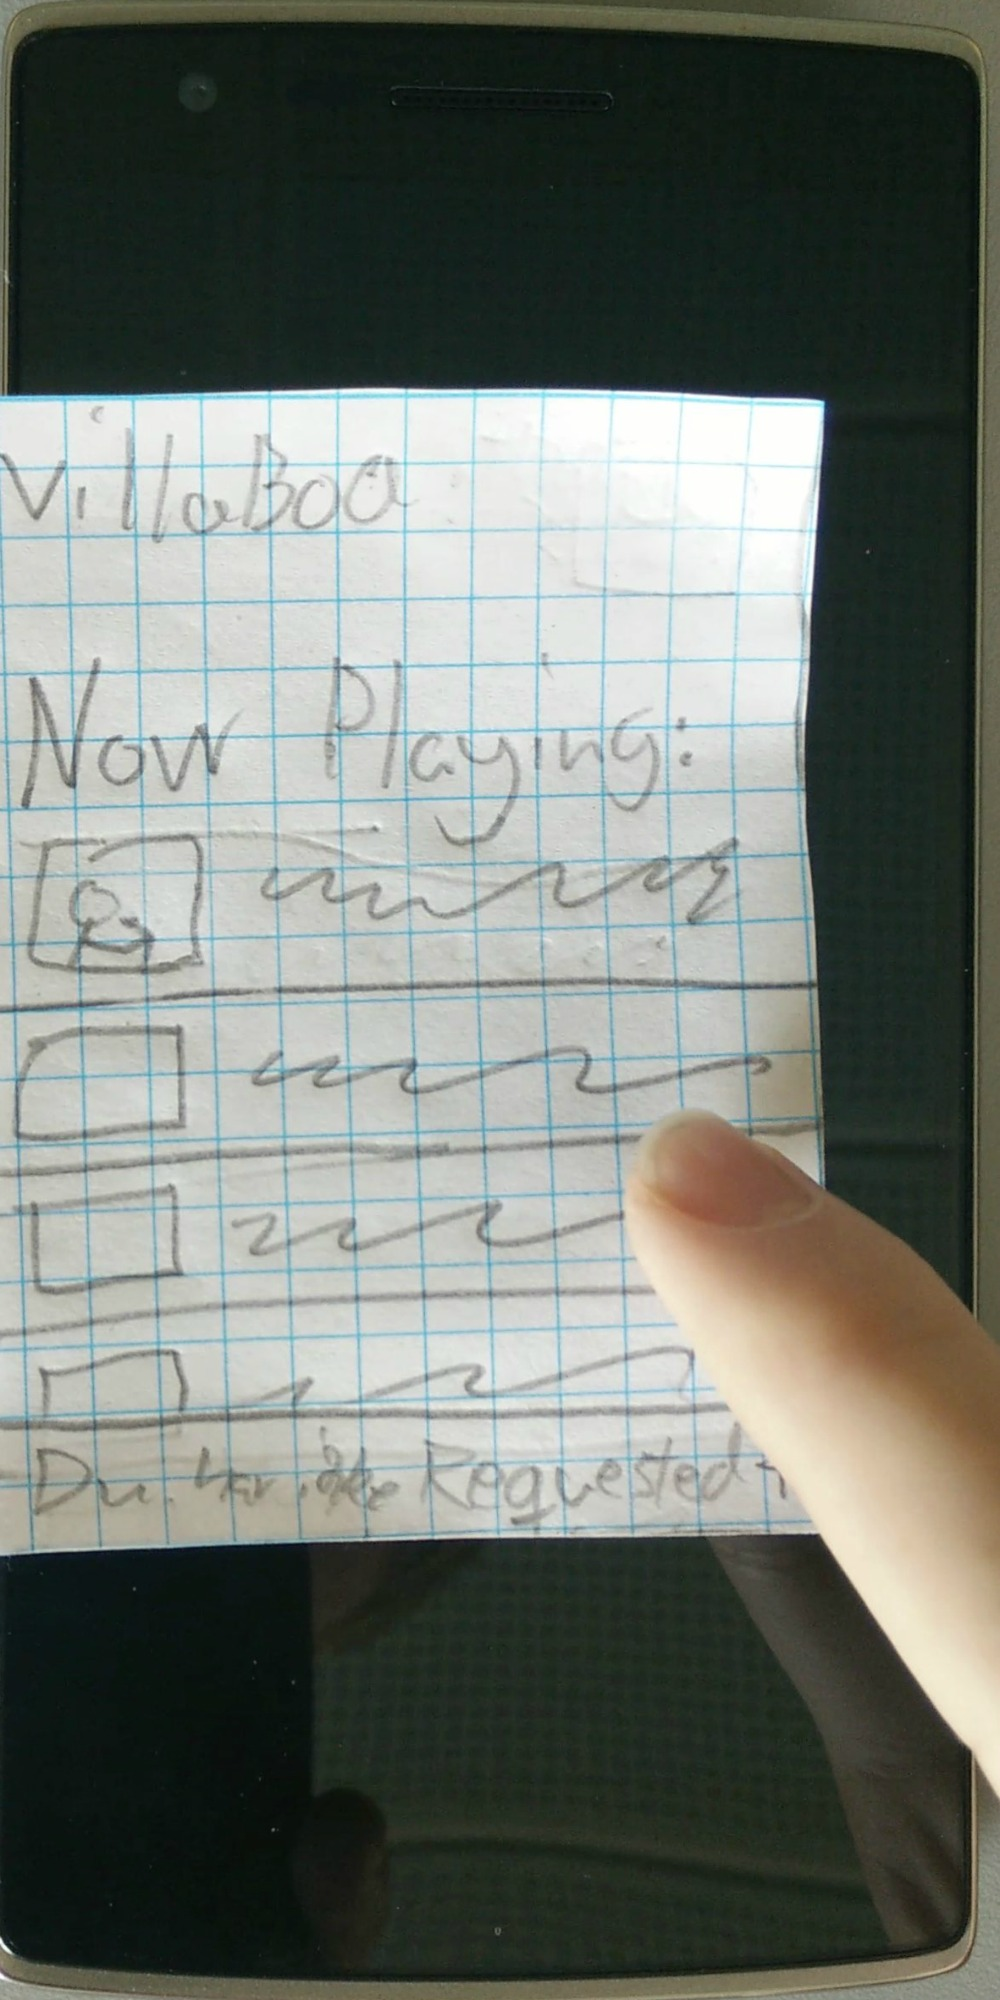
\includegraphics[width=\textwidth]{slides/Heider/paperPrototypeVoteInteraction}
		Papirprototype i design phase og i data indsamling en vertical prototype.
	\end{figure}
\end{frame}
\subsection{Usability test}
\begin{frame}{Usability test}
	\begin{figure}
		\centering
		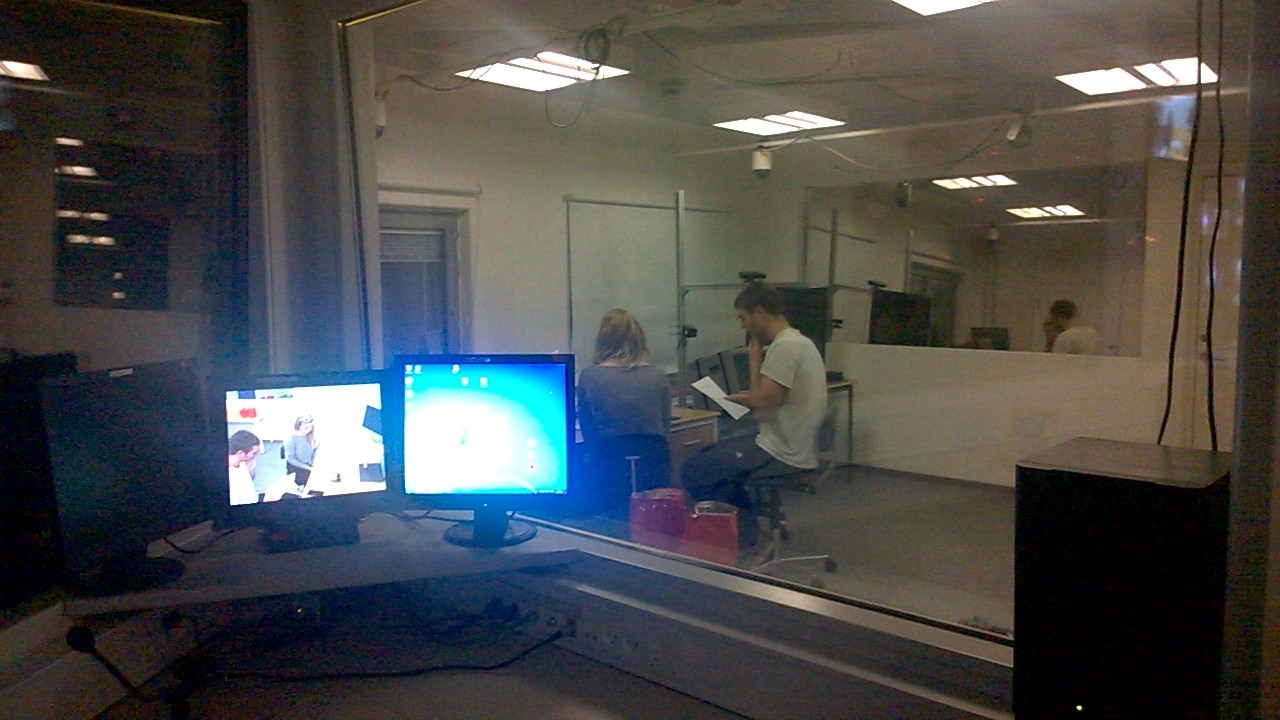
\includegraphics[width=\textwidth]{slides/Heider/subjectRoom}
	\end{figure}
	Hvordan vi gjorde det
	Videnssamling igennem: Instant Data Analysis - hvorfor vi brugte den
	\begin{itemize}
		\item hurtigt
		\item noget mere..
	\end{itemize}
\end{frame}
